\documentclass{beamer}
%
% Choose how your presentation looks.
%
% For more themes, color themes and font themes, see:
% http://deic.uab.es/~iblanes/beamer_gallery/index_by_theme.html
%
\mode<presentation>
{
  \usetheme{Madrid}      % or try Darmstadt, Madrid, Warsaw, ...
  \usecolortheme{beaver} % or try albatross, beaver, crane, ...
  \usefonttheme{serif}  % or try serif, structurebold, ...
  \setbeamertemplate{navigation symbols}{}
  \setbeamertemplate{caption}[numbered]
} 

\usepackage{hyperref}
\usepackage{tabu}
\usepackage[italian]{babel}
\usepackage[utf8]{inputenc}
\usepackage{pdfpages}
\usepackage{framed, color}
\definecolor{shadecolor}{rgb}{1,0.8,0.3}
\usepackage{color}
\usepackage[backend=bibtex, style=numeric,sorting=none]{biblatex}

\definecolor{pblue}{rgb}{0.13,0.13,1}
\definecolor{pgreen}{rgb}{0,0.5,0}
\definecolor{pred}{rgb}{0.9,0,0}
\definecolor{pgrey}{rgb}{0.46,0.45,0.48}

\usepackage{listings}
\lstset{language=Python,
  showspaces=false,
  showtabs=false,
  breaklines=true,
  showstringspaces=false,
  breakatwhitespace=true,
  commentstyle=\color{pgreen},
  keywordstyle=\color{pblue},
  stringstyle=\color{pred},
  basicstyle=\ttfamily,
  frame=lrbt,xleftmargin=\fboxsep,xrightmargin=-\fboxsep
}

\title[Ragazze Digitali 2019]{Ragazze Digitali A.A. 2018/2019}
\author{E. Salvucci - S. Gattucci - C. Varini}
\date{}

\AtBeginSection[]
{
  \begin{frame}<beamer>
    \frametitle{Outline}
    \tableofcontents[currentsection,currentsubsection]
  \end{frame}
}

\bibstyle{unsrt}
\bibliography{bibliography.bib}

\begin{document}

\setbeamertemplate{background}
{\includegraphics[width=\paperwidth,height=\paperheight]{images/ragazze_digitali.jpg}}
\begin{frame}
\end{frame}

\setbeamertemplate{background}
{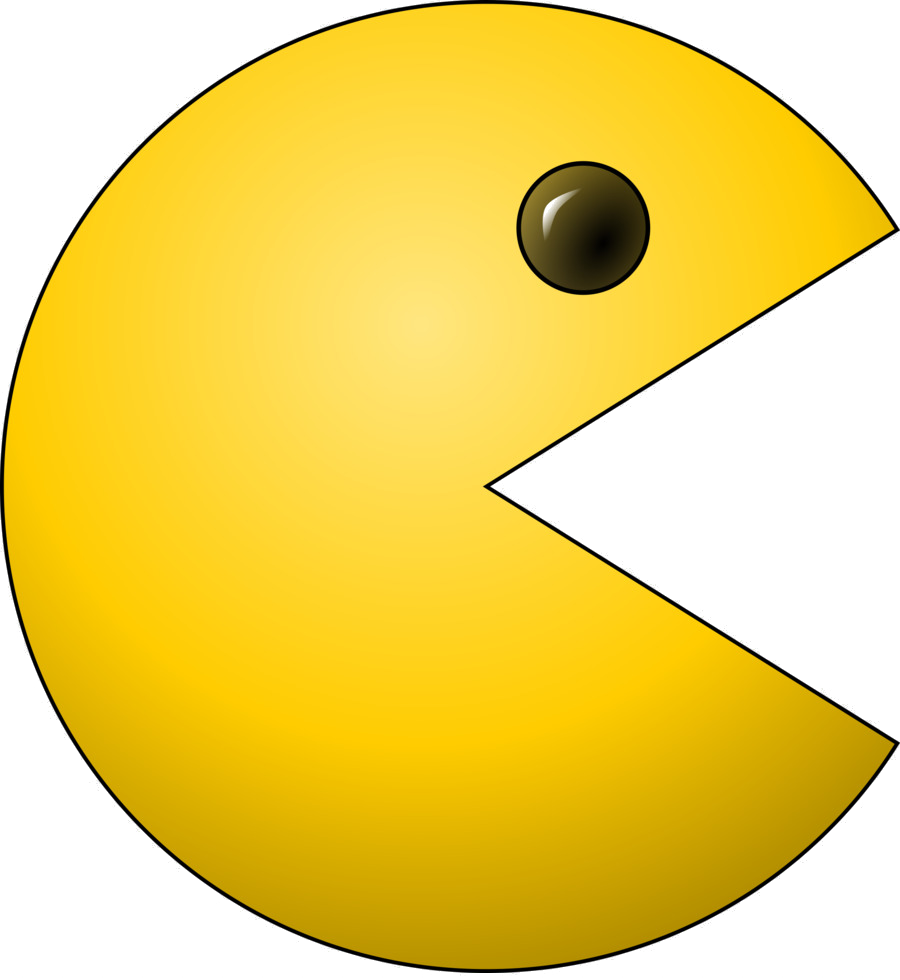
\includegraphics[width=\paperwidth,height=\paperheight]{images/pacman.jpg}}
\begin{frame}
\frametitle{Cosa faremo oggi}

\end{frame}

\setbeamertemplate{background}{}

\begin{frame}
\frametitle{Cosa faremo oggi}
Nel programma che faremo oggi il giocatore usera' le freccie della tastiera per muovere un quadrato nero (il nostro pacman) a destra, sinistra, in alto e in basso.

Ci saranno degli altri quadrati verdi (il cibo) che appariranno in posizioni casuali e che verranno "mangiati" dal quadrato nero quando questo li tocchera'.

Con il tasto ESC potremo uscire dal gioco e con il tasto X potremo teletrasportare il quadrato nero in una posizione random
\end{frame}

\section{Disegnamo la finestra di gioco e gli elementi al suo interno}

\begin{frame}[fragile]
    \frametitle{La finestra di gioco}
    
    \begin{lstlisting}
WINDOWWIDTH = 400
WINDOWHEIGHT = 400
windowSurface = pygame.display.set_mode((WINDOWWIDTH, WINDOWHEIGHT), 0, 32)
pygame.display.set_caption('Input')
    \end{lstlisting}
    
    \begin{block}{set\_mode(..)}
        \begin{itemize}
            \item La funzione set\_mode(resolution, flags, depth) inizializza una nuova finestra
            \item I suoi parametri:
                \begin{itemize}
                    \item resolution
                    \item flags
                    \item depth
                \end{itemize}
        \end{itemize}
    \end{block}

\end{frame}

\begin{frame}[fragile]
    \frametitle{La finestra di gioco}
    
    \begin{block}{set\_mode(..)}
        \begin{itemize}
            \item La funzione set\_mode(resolution, flags, depth) inizializza una nuova finestra
            \item I suoi parametri:
                
                \begin{itemize}
                    \item resolution: una coppia di numeri nella forma (0, 0) che rappresenta rispettivamente la larghezza e l'altezza della finestra
                    
                    \item flags: opzioni aggiuntive, alcuni esempi:
                    
                    pygame.FULLSCREEN    create a fullscreen display
                    pygame.RESIZABLE     display window should be sizeable

                    \item depth: profondita' di colori. Possiamo non preoccuparcene, se settato a 0 pygame decide il valore migliore per noi.
                \end{itemize}
        \end{itemize}
    \end{block}

\end{frame}

\begin{frame}[fragile]
    \frametitle{pygame.Rect(...)}
    disegna un rettangolo e lo memorizza nella variabile player.
    
    Quando dovremo cambiare il rettangolo che rappresenta il giocatore andremo a modificare questa variabile
\end{frame}    
    
\begin{frame}[fragile]
    \frametitle{pygame.Rect(...)}
    \begin{block}{pygame.Rect(X\_POSITION, Y\_POSITION, WIDTH, HEIGHT)}
        \begin{itemize}
            \item X\_POSITION: Posizione della coordinata x del rettangolo sulla finestra
            \item Y\_POSITION: Posizione della coordinata y del rettangolo sulla finestra
            \item WIDTH: Larghezza del rettangolo
            \item HEIGHT: Altezza del rettangolo
        \end{itemize}
    \end{block}
    \begin{lstlisting}
X_POSITION = 300
Y_POSITION = 100
WIDTH = 50
HEIGHT = 50
player = pygame.Rect(X_POSITION, Y_POSITION, 
                     WIDTH, HEIGHT)
    \end{lstlisting}
\end{frame}

\section{Gestione degli eventi}

\begin{frame}[fragile]
Pygame puo' generare eventi in seguito a input da tastiera da parte dell'utente.

\begin{block}{Eventi}
    \begin{itemize}
        \item QUIT: Evento generato quando il giocatore chiude la finestra di gioco.
        \item KEYDOWN: Evento generato quando il giocatore tiene premuto un tasto qualsiasi.
        \item KEYUP: Evento generato quando il giocatore rilascia un tasto qualsiasi che precedentemente stava tenendo premouto.
        \item MOUSEMOTION: Evento generato quando il mouse si muove all'interno della nostra finestra.
        \item MOUSEBUTTONDOWN: Evento generato quando viene premuto un tasto del mouse all'interno della nostra finestra
        \item MOUSEBUTTONUP: Evento generato quando viene premuto un tasto del mouse all'interno della nostra finestra
    \end{itemize}
\end{block}

\end{frame}

\section{Input da tastiera}

\begin{frame}[fragile]
    \frametitle{Input da tastiera}
    Settiamo 4 variabili, che rappresentano le diverse posizioni, con valori booleani inizialmente False.
    
    Quando il giocatore usera' il tasto sinistra cambieremo il valore corrispondente in True (e faremo lo stesso per gli altri tre tasti).
    
    Quando il giocatore lascera' il tasto premuto setteremo di nuovo il valore corrispondente a False
    \begin{lstlisting}
moveLeft = False
moveRight = False                                                                                                             
moveUp = False
moveDown = False 
    \end{lstlisting}
\end{frame}

\begin{frame}[fragile]
\frametitle{Gestire l'evento KEYDOWN}
Se l'evento scatenato e' KEYDOWN allora l'evento stesso ha un attributo chiamato "key" che indica quale tasto e' stato premuto.

\begin{lstlisting}
if event.type == KEYDOWN:
    if event.key == K_LEFT:
        moveRight = False
        moveLeft = True
    if event.key == K_RIGHT:
        moveLeft = False
        moveRight = True
    if event.key == K_UP:
        moveDown = False
        moveUp = True
    if event.key == K_DOWN:
        moveUp = False
        moveDown = True
\end{lstlisting}
    
\end{frame}

\begin{frame}{}
\frametitle{}
			\begin{figure}
   				\includegraphics[height=5cm]{images/constant_variables_for_keyboard_keys.png}
			\end{figure}
\end{frame}

\begin{frame}[fragile]
\frametitle{Gestire l'evento KEYUP}
Se l'evento scatenato e' KEYUP il nostro quadrato si dovra' fermare. Settiamo quindi la direzione del tasto rilasciato a False.

\begin{lstlisting}
if event.type == KEYUP:
    if event.key == K_ESCAPE:
        pygame.quit()
        sys.exit()
    if event.key == K_LEFT:
        moveLeft = False
    if event.key == K_RIGHT:
        moveRight = False
    if event.key == K_UP:
        moveUp = False
    if event.key == K_DOWN:
        moveDown = False
\end{lstlisting}
\end{frame}

\section{Input da mouse}

\begin{frame}[fragile]
\frametitle{Input da mouse}
    
    \begin{block}{Gestire eventi del mouse}
        \begin{itemize}
            \item MOUSEMOTION: Evento generato quando il mouse si muove all'interno della nostra finestra
            
            Ha degli attributi. In particolare ci sara' utile \textbf{pos}: Indica la posizione del mouse all'interno della finestra. La posizione e' rappresentata come tupla (x, y) dove x e y sono le coordinate del mouse.
            \item MOUSEBUTTONDOWN: Evento generato quando viene premuto un tasto del mouse all'interno della nostra finestra
            
            Ha degli attributi. In particolare ci sara' utile \textbf{button}: Indica quale tasto del mouse e' stato premuto.
            
            1 rappresenta il tasto sinistro, 2 il tasto centrale (se presente), 3 il tasto destro, 4 se la rotella e' stata mossa verso l'alto o 5 se mossa verso il basso.
            
            \item MOUSEBUTTONUP: Ha gli stessi attributi di MOUSEBUTTONDOWN.
        \end{itemize}
    \end{block}
    
\end{frame}

\section{Muovere il giocatore}

\begin{frame}[fragile]
\frametitle{Muovere il giocatore}

\begin{block}{Muovere il giocatore}
Se una delle 4 variabili, moveDown, moveUp, moveLeft o moveRight ha valore True dobbiamo muovere il nostro giocatore (memorizzato nella variabile player).

In particolare possiamo muovere il giocatore verso l'alto se questo non e' gia' arrivato all'estremo superiore della finestra, in basso se non e' arrivato a quello inferiore e cosi' via..

Per rappresentare il movimento cambieremo la posizione verso la quale ci vogliamo muovere aggiungendo o sottraendo un valore MOVESPEED (che rappresenta il quanto ci stiamo muovendo)
\end{block}

\begin{lstlisting}
if moveDown and player.bottom < WINDOWHEIGHT:
        player.top += MOVESPEED
    if moveUp and player.top > 0:
        player.top -= MOVESPEED
\end{lstlisting}
\end{frame}

\section{Disegnare il giocatore}

\begin{frame}[fragile]
\frametitle{Disegnare il giocatore}

Per adesso abbiamo solo detto, definendo player, quali sono le caratteristiche del nostro giocatore.

Non lo abbiamo ancora disegnato e mostrato a video

\begin{lstlisting}
pygame.draw.rect(windowSurface, BLACK, player)
\end{lstlisting}

\end{frame}

\section{Collision detection}

\begin{frame}[fragile]
\frametitle{Collision detection}

\begin{block}{player.colliderec()}
Andiamo a rilevare le collisioni tra il giocatore (player) e i cibi (foods).
Utilizziamo la funzione colliderect che verifica se due rettangoli si toccano.
\end{block}

\begin{lstlisting}
new_foods = foods
for food in foods:
    if player.colliderect(food):
        foods.remove(food)
new_foods = []
\end{lstlisting}

\end{frame}

\section{Clock e display.update()}

\begin{frame}[fragile]
\frametitle{pygame.display.update()}

\begin{block}{pygame.display.update()}

Le proprieta' del nostro giocatore sono cambiate, come anche quelle dei cibi. Il giocatore e' stato spostato, alcuni cibi rimossi e alcuni aggiunti.

E' necessario aggiornare la finestra di gioco con le nuove caratteristiche di giocatore e cibi.
\end{block}

\begin{lstlisting}
    pygame.display.update()
\end{lstlisting}

\end{frame}

\begin{frame}[fragile]
\frametitle{Clock}

\begin{block}{Clock}
Inizializziamo, all'inizio del nostro programma, una variabile globale chiamata mainClock che ci aiutera' (in generale) a tenere traccia del passare del tempo.
\end{block}

\begin{lstlisting}
mainClock = pygame.time.Clock()
\end{lstlisting}
\end{frame}

\begin{frame}[fragile]
\frametitle{pygame.time.tick(..)}

\begin{block}{pygame.time.tick(..)}
come ultima riga del while utilizziamo la funzione tick(..) che, lascia scorrere del tempo tra una chiamata e l'altra della funzione stessa. Quindi, secondo l'esempio, dopo il primo passeranno 40 millisecondi prima che venga eseguito di nuovo il tick.
\end{block}

\begin{lstlisting}
mainClock.tick(40)
\end{lstlisting}

\begin{block}{}
Perche' questo?

Proviamo a togliere la riga mainClock.tick(40)
\end{block}

\end{frame}

\begin{frame}[fragile]
\frametitle{E' il vostro turno}

\begin{block}{E' il vostro turno!}
Prendiamo come riferimento il codice al \href{https://raw.githubusercontent.com/ragazzedigitalicesena/slide-2019/master/tex/chapter_19-20/collisionDetection.py}{link}, potete copiarlo

\href{https://raw.githubusercontent.com/ragazzedigitalicesena/slide-2019/master/tex/chapter_19-20/collisionDetection.py}{Download}

\vspace{5mm}
Completiamo il codice fornito secondo le indicazioni della pagine successive.
\end{block}

\end{frame}

\begin{frame}[fragile]
\frametitle{E' il vostro turno - Parte 1}
\begin{block}{E' il vostro turno!}
    \begin{itemize}
        \item Crea una variabile che contenga, inizialmente, una lista vuota (chiamandola foods)
        \item Crea anche una costante chiamata FOODSIZE che rappresentera' sia la larghezza sia l'altezza del cibo (dandole il valore che preferisci, per il giocatore avevamo usato 50)
    \end{itemize}{}
\end{block}
\end{frame}

\begin{frame}[fragile]
\frametitle{E' il vostro turno - Parte 1}
\begin{block}{E' il vostro turno!}
    \begin{itemize}
        \item Con un ciclo for (che si ripeta 20 volte, aiuto: range(20)) aggiungiamo alla lista foods  (aiuto: append(..)) dei rettangoli che rappresenteranno i "cibi" del nostro gioco.
        
        Usiamo pygame.Rect(..) come visto nell'esempio con cui abbiamo creato il rettangolo per il giocatore.
        
        La larghezza e l'altezza del rettangolo sara' FOODSIZE.
        \item Prima abbiamo usato X\_POSITION e Y\_POSITION per posizionare il rettangolo del giocatore. In questo caso usa un numero generato casualmente compreso tra 0 e la larghezza della finstra WINDOWWIDTH - FOODSIZE (con random.randint(..) come abbiamo visto)
    \end{itemize}{}
\end{block}
\end{frame}

\begin{frame}[fragile]
\frametitle{E' il vostro turno - Parte 2}
\begin{block}{E' il vostro turno!}
    Abbiamo visto come gestire eventi generati dalla pressione e dal rilascio dei tasti su, giu, destra o sinistra.
    
    Dai la possibilita' all'utente di usare \textbf{anche} le lettere \textbf{W} per muoversi verso l'alte, \textbf{S} verso il basso, \textbf{A} verso sinistra e \textbf{D} verso destra (quindi o le frecce o le lettere).
    
    \begin{lstlisting}
    event.key == K_w
    # Per la pressione del tasto W
    event.key == K_s
    # Per la pressione del tasto S
    event.key == K_a
    # Per la pressione del tasto A
    event.key == W_d
    # Per la pressione del tasto D
    \end{lstlisting}
\end{block}

\end{frame}

\begin{frame}[fragile]
\frametitle{E' il vostro turno - Parte 3}
\begin{block}{E' il vostro turno!}
    Ora vogliamo dare la possibilita' al giocatore di essere teletrasportato in una posione casuale alla pressione del tasto X
    
    Aggiungi la gestione dell'evento "pressione del tasto X" agli if di keyup.
    
    \begin{lstlisting}
# per teletrasportare il giocatore in una
# posizione random usa, dentro all'if:
player.top = random.randint(0, WINDOWHEIGHT - player.height)
player.left = random.randint(0, WINDOWWIDTH - player.width)
    \end{lstlisting}
\end{block}

\end{frame}

\begin{frame}[fragile]
\frametitle{E' il vostro turno - Parte 4}
\begin{block}{E' il vostro turno!}
    Aggiungi un "cibo" nella posizione in cui si trovava il mouse al momento della pressione del tasto sinistro (la pressione in questo caso non ci interessa, ci interessa solo il rilascio MOUSEBUTTONUP)
        
    Lo si puo' fare prendendo spunto dall'esempio in cui abbiamo aggiunto i cibi in posizione random. In questo caso li aggiungeremo nella posizione del mouse (elementi 0 e 1 della lista event.pos[0]).
\end{block}

\end{frame}

\begin{frame}[fragile]
\frametitle{E' il vostro turno - Parte 5}
\begin{block}{E' il vostro turno!}
Abbiamo visto come muovere il giocatore verso l'alto e verso il basso. Seguendo quell'esempio aggiungi il movimento verso sinistra e verso destra (le posizioni sinistra e destra del giocatore sono rispettivamente player.left e player.right) 
\end{block}

\end{frame}

\begin{frame}[fragile]
\frametitle{E' il vostro turno - Parte 6}
\begin{block}{E' il vostro turno!}
Analogamente a come abbiamo disegnato e mostrato a video il quadrato del giocatore, mostra a video/disegna i quadrati di tutti i food presenti nella lista foods
\end{block}

\end{frame}

\begin{frame}[fragile]
\frametitle{E' il vostro turno - Parte 7}
\begin{block}{E' il vostro turno!}
La funzione \textbf{ pygame.time.get\_ticks() } restituisce il tempo (in millisecondi) trascorso da quando e' stato avviato pygame (e quindi, nel nostro caso, il programma).

\vspace{5mm}
Come possiamo fare un countdown del tempo       ?
Prova a farlo stampando il tempo con una print

Ad esempio:
\begin{itemize}
    \item 10 s
    \item 9 s
    \item 8 s 
    \item ...
\end{itemize}
\end{block}

\end{frame}

\begin{frame}

\begin{center}
    \bigskip
    Materiale rilasciato con licenza
    
    \textbf{\href{http://creativecommons.org/licenses/by-sa/4.0/}{Creative Commons - Attributions, Share-alike 4.0}}
    
    \medskip
    \includegraphics[height=0.8cm]{images/cc.png}
\end{center}

\end{frame}

\end{document}